\chapter{Desarrollo}
\label{chap:desarrollo}

En este capítulo se explicará todo el proceso de desarrollo.


\section{Mockup: versión 0.1}

El paso previo antes de comenzar con un desarrollo profundo consistió en comprobar que las herramientas que se querían usar servían para el propósito propuesto.
Fue así que la primera versión ``usable'' del proyecto consistió en un botón con el que se podía interactuar.
Al hacerlo, se mostraría un menú que permitiría añadir nuevos botones, conectados por líneas, formando una estructura con forma de árbol.
Esto sería exportado a formato web y se desplegaría en GitHub Pages.

Para iniciar este proceso, primero hizo falta hacer un análisis de la forma en la que se estructura Godot.
Esto se explica en la Sección \ref{sec:herramientas_godot}.


%\subsection{Godot: el motor y sus componentes estructurales}

\subsection{Primeras escenas}

La primera escena que se creó fue el menú principal.
Al ya esperar crear varios algoritmos, era una escena simple de la que había que partir.
En ella se instanció un botón (un nodo de tipo Control (interfaz) caracterizado por emitir una señal cuando es pulsado) con el texto que cambiaba a la escena donde se encontraba el árbol.
En la Figura \ref{fig:primera_version_del_main_menu} se ve este menú principal.

\begin{figure}[hp!]
  \centering
  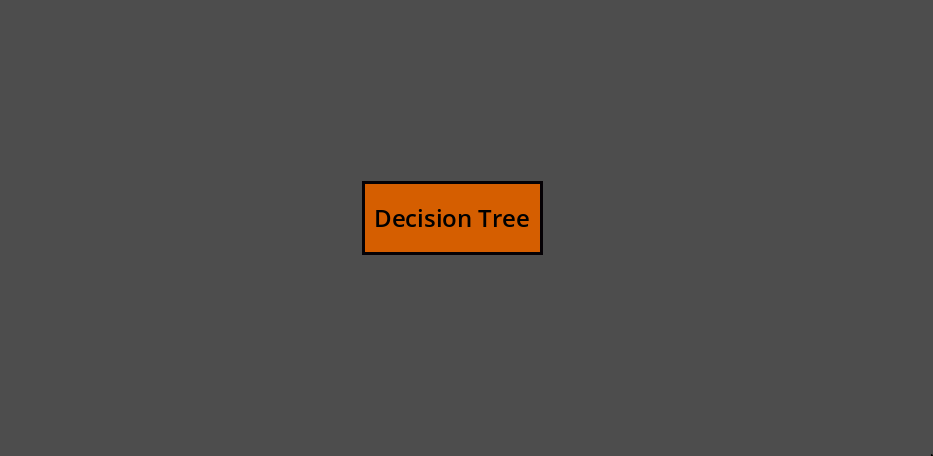
\includegraphics[width=0.75\textwidth]{imaxes/primera_version_del_main_menu.png}
  \caption{Versión preliminar del menú principal.}
  \label{fig:primera_version_del_main_menu}
\end{figure}

Al pulsar el botón se cambiaba de escena a una en la que se encontraba una entidad de una clase personalizada, el ``DNode''.
Esta clase heredaba de la clase botón y tenía tres atributos más: ``id'', ``parent\_id'', y ``sons\_id''.
Los primeros eran enteros, y el segundo un Array de enteros.
Al hacerle clic se desplegaba un menú con una opción: añadir nodo hijo.
Seleccionarla hacía aparecer un nuevo botón debajo del anterior, conectado por una línea.
Esto se podía hacer cuantas veces se quisiera, y hacía que fueran apareciendo nuevos nodos hijo, que se colocaban uno al lado de otro.
Estos siguientes botones tenían una segunda opción en el menú: eliminar nodo.
Esto eliminaba el nodo y sus hijos.

Por debajo el árbol era un diccionario.
Las claves eran enteros, correspondientes a los ids de los DNodes, y los valores eran los propios DNodes.
Estos eran conectados con otros nodos y colocados en pantalla en base a sus atributos de ``parent\_id'' y ``sons\_id''.

Además, en la escena había otros dos botones arriba a la derecha.
En este momento no hacían nada; eran el inicio de lo que acabaría siendo la funcionalidad de cargar y guardar el árbol, retomada durante el desarrollo del árbol de decisión.
En la Figura \ref{fig:primera_version_arbol} se puede ver el estado de esta primera escena interactiva.

\begin{figure}[hp!]
  \centering
  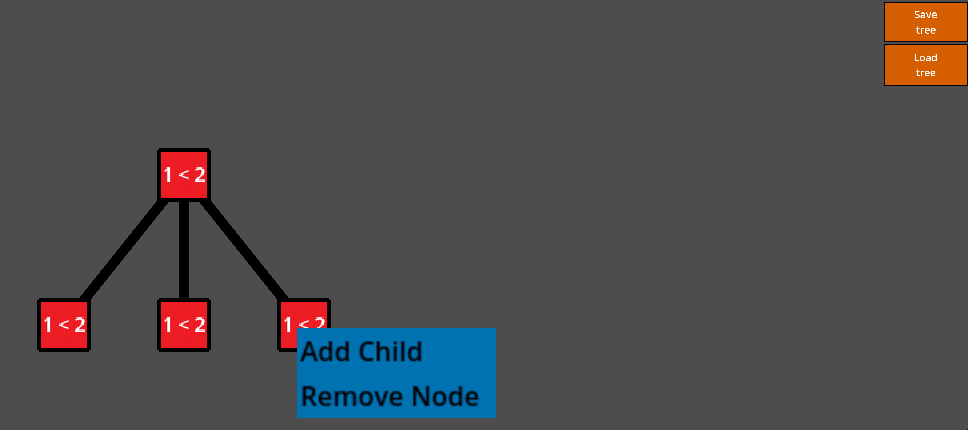
\includegraphics[width=0.75\textwidth]{imaxes/primera_version_arbol.png}
  \caption{Primera escena de prueba para ver el funcionamiento del árbol.}
  \label{fig:primera_version_arbol}
\end{figure}


\subsection{Exportación web con GitHub Pages}

Con esta versión funcional, faltaba probar a exportar a web para comprobar que Godot servía como motor de desarrollo para la aplicación web.
En Godot, para exportar el proyecto a HTML5, hay que descargar las plantillas de exportación, las cuales proporcionan el entorno web base y un archivo HTML que contiene en su estructura el elemento ``<canvas>'', donde el motor (compilado en WebAssembly) inicializa el renderizado gráfico y captura la interactividad.
La prueba se completó sin problemas con un proyecto tan simple.
Más adelante se exploran configuraciones más complejas de la exportación web debido a la creación del plugin para el renderizado de fórmulas.

Después se configuró desde la interfaz web de GitHub la funcionalidad de GitHub Pages.
Para ello, accedí desde la configuración del repositorio a la ventana ``Pages'', desde la cual se puede seleccionar una rama de publicación (para este caso se seleccionó ``main'') y una carpeta para ser la raíz de la página web (en este caso, la carpeta ``docs'', la predeterminada).
Con esta función activada, hubo que exportar el proyecto a la carpeta indicada.
Una vez subidos los cambios a la rama ``main'', la aplicación estaba desplegada.



\section{Árbol de decisión: versión 0.2}

El proyecto dejó de ser un simple mockup cuando se comenzó a trabajar en el primer algoritmo: el árbol de decisión.

\subsection{Primera arquitectura del árbol}

Para comenzar el desarrollo del árbol de decisión, el primer objetivo fue separar la prueba visual inicial de una estructura que pudiera sostener más adelante un algoritmo real. La primera versión del árbol, descrita en la sección anterior, servía para crear nodos manualmente y para comprobar que Godot permitía representar una estructura jerárquica en una escena interactiva. A partir de ese punto se empezó a transformar esa prueba en una vista específica de árbol, con sus propias escenas, scripts y responsabilidades.

La escena principal del proyecto quedó configurada en Godot como un menú simple, implementado como un nodo de tipo ``Control''. Este menú contenía un único botón que al pulsarse llamaba a ``change\_scene\_to\_file'' para cargar la escena del árbol. De esta manera, el menú principal podía crecer en el futuro sin mezclar su lógica con la representación del árbol.

La vista del árbol se organizó dentro de un nodo Control de tipo ``ScrollContainer''.
Este nodo está pensado para tener un solo hijo de tipo Control, y habilita que cuándo este es más grande que la zona que tiene asignada, se pueda scrollear para mover el contenido.
Esta decisión fue importante desde el principio, porque un árbol puede crecer en anchura y altura con rapidez.
Si todos los nodos se colocasen directamente sobre una escena fija, bastarían unos pocos niveles para que parte del árbol quedase fuera de pantalla.
Por ello se creó un ``DTreeCanvas'', el nodo hijo del ScrollContainer, que instanciaba la escena del árbol.
Su función era calcular el tamaño mínimo necesario para contener la estructura completa.
El cálculo partía de los límites del árbol, obtenidos mediante ``get\_tree\_bounds'', y ajustaba ``custom\_minimum\_size'' para que el ScrollContainer pudiera desplazarse hasta todas las zonas relevantes.
%%Dudas: pongo en esta parte que había un nodo de godot que ya me ayudaba con esto, o ya lo digo más adelante?

El núcleo visual del árbol se encapsuló en la clase ``DTreeLogical''.
En su primera versión esta clase heredaba de ``Node2D'' y mantenía un diccionario ``nodes\_dict'', donde cada clave era el identificador de un nodo y cada valor era la instancia visual correspondiente.
También guardaba ``root\_id'', que apuntaba al nodo raíz.
Al iniciarse, el árbol creaba una raíz con identificador 0, la añadía al contenedor de nodos y ejecutaba un reposicionamiento completo.
Esta estructura basada en diccionario permitía acceder a cualquier nodo por su identificador sin recorrer toda la escena de Godot.

El posicionamiento se resolvió mediante un recorrido en orden.
Cada nodo guardaba su profundidad y un índice ``inorder\_index''.
Las hojas recibían índices consecutivos, y los nodos internos se colocaban en el punto medio entre el primer y el último hijo.
Después, ``\_apply\_positions'' multiplicaba esos índices por dos constantes de espaciado, una horizontal y otra vertical.
Con ello se conseguía una distribución simple, estable y suficiente para las primeras pruebas: los hijos aparecían por debajo del padre, y el padre quedaba centrado respecto a ellos.
Tras cada modificación se llamaba a ``relayout\_tree'', que recalculaba índices, posiciones y conexiones.

Las conexiones se implementaron como una escena independiente, ``Conection'', basada en ``Line2D''. En un primer momento la línea solo unía las posiciones globales del nodo padre y del nodo hijo. Más adelante se adaptó para trabajar con nodos de tipo ``Control'', tomando el centro visual de cada botón y convirtiendo esas posiciones al espacio local de la conexión. El contenedor de conexiones recorría ``nodes\_dict'', comprobaba los hijos de cada nodo mediante ``sons\_id'' y creaba una línea por cada relación padre-hijo. Esta separación evitaba que los nodos tuviesen que dibujar sus propias ramas y dejó la responsabilidad de las aristas concentrada en una escena concreta.

El nodo del árbol, ``DNode'', también cambió durante esta primera fase. La versión inicial era un ``Node2D'' con un ``Sprite2D'', un ``Area2D'' y una ``CollisionShape2D''. El ``Area2D'' recibía eventos de ratón, cambiaba el color del sprite al pasar el cursor y abría un menú contextual al hacer clic. Esta solución funcionaba para una prueba gráfica, aunque obligaba a gestionar manualmente colisiones, sprites y etiquetas. En el refactor posterior el nodo pasó a heredar directamente de ``Button''. Con esto se aprovechó el sistema de interfaz de Godot, incluyendo eventos ``gui\_input'', texto incorporado, temas y tamaños de control.

El ``DNode'' conservó las variables necesarias para representar la estructura: ``id'', ``parent\_id'', ``sons\_id'', ``depth'' e ``inorder\_index''. A ellas se añadieron variables relacionadas con el aprendizaje automático, como ``attribute'', ``label'', ``is\_leaf'' y ``branch\_value''. Aunque al principio muchas de ellas todavía no se usaban para ejecutar un algoritmo completo, dejaban preparado el nodo para distinguir entre nodos internos, que representan atributos de división, y nodos hoja, que representan etiquetas de clasificación. También se mantuvo ``can\_remove'', usado para impedir que la raíz pudiese eliminarse desde el modo manual.

La interacción manual quedó coordinada por ``ControllerDTree''. El controlador recibía referencias al árbol, al canvas y a la vista, calculaba el siguiente identificador disponible y conectaba la señal ``change\_child\_requested'' de cada ``DNode''. Cuando un nodo solicitaba añadir un hijo, el controlador instanciaba un nuevo ``DNode'', le asignaba identificador, padre y profundidad, lo añadía a ``nodes\_dict'', lo insertaba en el contenedor visual y registraba su identificador en ``sons\_id'' del padre. Cuando se solicitaba eliminar un nodo, el controlador borraba recursivamente todo su subárbol. Para ello duplicaba la lista de hijos antes de iterar, evitando modificar el array original durante el recorrido, eliminaba el identificador del hijo en el padre, retiraba el nodo del diccionario y liberaba la instancia visual con ``queue\_free''.

En paralelo se crearon dos escenas auxiliares para cargar y guardar árboles. En esta fase eran una funcionalidad preliminar, basada en serializar los atributos estructurales de cada nodo a un archivo JSON en ``user://tree.json''. El guardado recorría ``nodes\_dict'' y extraía identificador, padre, hijos, profundidad e índice de orden. La carga hacía el proceso inverso: leía el JSON, reconstruía instancias de ``DNode'', rellenaba sus atributos y las añadía a un nuevo árbol. Aunque esta persistencia se revisaría bastante más tarde, ya muestra que desde el inicio se pensaba en el árbol como una estructura de datos reconstruible, no solo como elementos colocados manualmente en una escena.

El siguiente cambio relevante fue la preparación del modo automático. El controlador dejó de limitarse a gestionar edición manual y empezó a recibir un modo de funcionamiento, ``manual'' o ``automatic''. En modo manual seguía conectando señales de nodos y permitiendo crear o borrar ramas. En modo automático creaba un panel de control, ``PanelAlgorithmDTree'', con botones para iniciar entrenamiento y avanzar al siguiente paso. Este panel se añadía sobre la vista principal y conectaba sus botones con métodos del controlador. La interfaz todavía era sencilla, con ``Start Training'' y ``Next Step'', y ya introducía el flujo que se mantendría durante el desarrollo: el usuario avanza el algoritmo paso a paso desde la interfaz.

Para ese modo automático se creó la clase ``AlgorithmDTree''. Su primera responsabilidad fue implementar una versión básica de ID3 sobre datos categóricos. El algoritmo guardaba los datos de entrenamiento, la lista de atributos disponibles, una referencia al árbol visual y una pila de llamadas, ``call\_stack'', que permitía convertir una construcción recursiva en una ejecución incremental. Cada contexto de la pila contenía el subconjunto de datos correspondiente, los atributos restantes, el identificador del padre, el valor de la rama por la que se llegaba a ese nodo, la profundidad y un identificador visual todavía pendiente.

El método ``start\_training'' inicializaba el estado y añadía a ``call\_stack'' el contexto de la raíz. A partir de ahí, cada pulsación en ``Next Step'' ejecutaba ``next\_step'', que extraía un contexto de la pila y llamaba a ``\_build\_node\_step''. Esta función concentraba la lógica de decisión. Primero obtenía las etiquetas de los datos. Si todas eran iguales, pedía crear un nodo hoja con esa clase. Si no quedaban atributos, calculaba la clase mayoritaria y creaba una hoja de mayoría. En el resto de casos calculaba la ganancia de información para cada atributo, seleccionaba el atributo con mayor ganancia, preparaba un contexto por cada valor posible del atributo elegido y solicitaba crear un nodo interno.

La entropía se calculó directamente en GDScript. La función ``\_entropy'' contaba ocurrencias de cada etiqueta, transformaba cada conteo en una probabilidad y acumulaba la expresión $-p \log_2(p)$. Sobre esa función se construyó ``\_information\_gain'', que calculaba la entropía total del conjunto, dividía los datos por el valor del atributo y restaba la entropía ponderada de los subconjuntos. Esta implementación fue deliberadamente explícita. En lugar de delegar en una biblioteca externa, el código mostraba de forma transparente los mismos cálculos que después debían explicarse en la interfaz.

La coordinación entre el algoritmo y la escena visual se hizo mediante señales. ``AlgorithmDTree'' emitía ``add\_node\_requested'' indicando padre, valor de rama, atributo, etiqueta y si el nodo era hoja. El controlador recibía esa señal y decidía si debía crear la raíz o un hijo. Para los nodos hijos, actualizaba ``branch\_value'' con el valor del atributo que llevaba hasta ese nodo. Esta variable se usaría poco después para mostrar etiquetas en las conexiones. Como los contextos de los hijos se añadían a la pila antes de saber el identificador real del nodo padre, se introdujo el valor temporal ``-2'' para marcar padres pendientes. Cuando el controlador terminaba de crear un nodo, llamaba a ``update\_pending\_parent\_ids'', que sustituía esos padres pendientes por el identificador recién creado.

Este primer modo automático aún tenía datos de entrenamiento definidos en el propio controlador. El conjunto de prueba contenía frutas descritas mediante atributos categóricos como ``color'', ``shape'' y ``size'', y una columna ``class''. Aunque era un dataset muy pequeño, cumplía dos funciones. Permitía comprobar que la lógica ID3 generaba nodos y ramas, y permitía observar si el árbol visual se actualizaba correctamente en cada paso. A partir de aquí el problema principal dejó de ser crear nodos a mano y pasó a ser sincronizar tres niveles: el estado del algoritmo, la estructura lógica del árbol y la escena que veía el usuario.


\subsection{Reorganización de la vista y primeros elementos explicativos}

Una vez creada la primera versión automática, se reorganizó la escena del árbol para reducir rutas frágiles y separar mejor las responsabilidades. La carpeta inicial ``scenes/views/dtree'' se sustituyó por ``scenes/views/dtree\_view'', y el controlador se movió fuera de la vista, a ``scenes/controllers/controller\_dtree''. Este cambio tenía un objetivo práctico: convertir el controlador en un componente de coordinación capaz de comunicarse con el árbol, la vista, el algoritmo y, más adelante, la ventana informativa.

Durante esta reorganización se probó una estructura con ``SubViewport'' y ``SubViewportContainer'' para poder aplicar zoom al árbol con ``Ctrl'' y la rueda del ratón. La escena contenía un panel inicial con dos opciones, creación manual y creación algorítmica, y el árbol se encontraba dentro de un viewport colocado dentro del ``ScrollContainer''. Esta versión llegó a incluir variables como ``zoom\_level'', ``min\_zoom'', ``max\_zoom'' y ``zoom\_step''. El enfoque añadía complejidad a la entrada de usuario y a los tamaños de la vista. Poco después se retiró esa capa de viewport y el ``DTree'' pasó a ser hijo directo del ``ScrollContainer''. Así se mantuvo el desplazamiento por la vista sin añadir una transformación extra sobre el árbol.

La eliminación del canvas intermedio obligó a revisar el centrado del árbol. En Godot, un ``ScrollContainer'' controla la posición de sus hijos, así que desplazar el propio ``DTree'' no ofrecía un resultado estable. La solución fue mover internamente las posiciones de los nodos. El método ``update\_canvas\_size\_and\_center'' quedó dentro de ``DTreeLogical'', calculando primero el rectángulo de ocupación del árbol, después el tamaño final necesario y, por último, un desplazamiento aplicado a cada nodo. Con este desplazamiento, el contenido del árbol quedaba centrado dentro del área de scroll. Después se actualizaba ``custom\_minimum\_size'' para que las barras del ``ScrollContainer'' conociesen el nuevo tamaño navegable.

También se tuvo en cuenta que el ``ScrollContainer'' actualiza sus barras después de una pasada de layout. Por ese motivo, al centrar el árbol se usó ``set\_deferred'' sobre ``scroll\_horizontal'' y ``scroll\_vertical''. Esta decisión evitaba que Godot limitase el desplazamiento a los valores antiguos justo después de cambiar el tamaño mínimo. Es un detalle pequeño, con un efecto importante para que la vista quedase centrada al crear o modificar el árbol y no apareciese desplazada a una esquina.

La escena ``DTreeView'' empezó a actuar como punto de entrada del flujo de árbol. En ``\_ready'' conectaba los botones del panel de selección, ocultaba el ``ScrollContainer'' y el menú del árbol, y solo mostraba el panel inicial. Al escoger modo manual, hacía visible el árbol, activaba el menú con los botones de carga y guardado, configuraba ``DTreeLogical'' en modo ``manual'' e inicializaba el controlador. Al escoger modo algorítmico, hacía visible el árbol y la ventana, creaba una instancia de ``AlgorithmDTree'', la añadía a la escena y entregaba esa referencia al controlador. Con ello la vista dejó de ser una escena pasiva y pasó a gestionar un flujo de usuario: primero elegir modo, después interactuar con el árbol.

En esta misma fase se creó el autoload ``Constants''. Este script centralizaba identificadores de escenas y temas en dos diccionarios, ``SCENES'' y ``THEMES''. En vez de repetir rutas o UID en scripts distintos, el controlador, el árbol, el menú principal y las conexiones podían acudir a ``Constants.SCENES'' para instanciar escenas como ``dnode'', ``controller\_dtree'', ``panel\_algorithm\_dtree'' o ``conection''. En un proyecto Godot que cambia de carpetas durante el desarrollo, esta centralización reduce errores al mover escenas, porque las referencias se corrigen en un único punto.

La representación visual de los nodos ganó una primera distinción semántica mediante temas. Se añadieron dos recursos ``Theme'': uno para nodos hoja y otro para nodos internos. El tema de hoja usaba una forma más redondeada y un color verdoso, mientras que el tema de nodo interno usaba un color rojizo y esquinas menos redondeadas. ``DNode'' precargaba ambos temas desde ``Constants.THEMES'' y en ``\_ready'' aplicaba uno u otro según ``is\_leaf''. Esta separación hacía que la estructura del árbol se entendiese con menos lectura: los nodos que clasifican y los nodos que dividen los datos tenían una apariencia distinta.

El mismo cambio introdujo ``was\_created\_by\_algorithm''. Los nodos creados por el algoritmo marcaban esta variable a ``true'', y ``DNode'' solo conectaba el menú contextual si el nodo no había sido creado por el modo automático. Esta decisión evitaba que el usuario modificase manualmente nodos que formaban parte de una ejecución algorítmica. El modo manual y el modo automático compartían la misma escena de nodo, aunque su comportamiento frente a clics era distinto. Así se reutilizaba la representación visual sin permitir ediciones que rompiesen la coherencia del entrenamiento paso a paso.

El panel algorítmico también se ajustó a una interfaz más cercana al idioma de la aplicación. Los botones pasaron de ``Start Training'' y ``Next Step'' a ``Empezar entrenamiento'' y ``Siguiente paso''. Además se añadió un botón ``Detalle'', inicialmente poco usado, que anticipaba la necesidad de abrir o actualizar información complementaria. En el controlador se añadieron señales propias, ``next\_step'' y ``detail'', de forma que el botón de siguiente emitía una señal del controlador y esta se conectaba al método ``next\_step'' del algoritmo. Esto desacoplaba la interfaz del algoritmo: el botón ya no llamaba directamente al objeto de entrenamiento.

El nombre del controlador también se corrigió de ``AlgDTree'' a ``ControllerDTree''. Aunque pueda parecer un cambio menor, aclara la responsabilidad de la clase. El algoritmo vive en ``AlgorithmDTree'', mientras que ``ControllerDTree'' se ocupa de conectar botones, señales, nodos visuales, árbol y ventana. Esta separación fue ganando valor en los commits posteriores, porque cada avance del algoritmo requería actualizar la escena, recalcular posiciones, refrescar la ventana o cambiar estados de botones.

Otro cambio de esta etapa fue la creación de una ventana informativa. Primero se añadió directamente como un nodo ``Window'' dentro de ``DTreeView'', con un ``RichTextLabel'' que mostraba el mensaje inicial ``Presiona el botón \"Empezar entrenamiento\"''. Después se extrajo a su propia escena, ``scenes/interface/window/window.tscn'', con su script ``window.gd''. Esta extracción era necesaria para que la ventana tuviese su propia lógica, sus plantillas de texto y su método de actualización, sin llenar ``DTreeView'' de código explicativo.

La ventana comenzó con una posición a la derecha del árbol, cerca de ``(800, 200)'', y después se movió a ``(20, 150)'' con un tamaño de ``300 x 350''. El ajuste mantuvo la lógica y muestra una preocupación temprana por la composición de la escena. La ventana debía estar visible durante el entrenamiento y ocupar un lugar que no estorbase demasiado a la lectura del árbol. En estas primeras versiones seguía siendo una ventana flotante de Godot, bastante distinta de los paneles integrados que se adoptarían más adelante.

El primer contenido de la ventana se construyó con plantillas de texto. ``window.gd'' definía un diccionario ``template\_texts'' con tres casos: ``internal'', ``leaf'' y ``leaf\_mayority''. El texto de nodo interno explicaba cuántos datos habían llegado por la rama, qué etiquetas tenían, qué atributos quedaban, qué métrica se usaba para decidir la división, qué valores obtuvo cada atributo y qué ramas se crearían a partir del mejor atributo. El texto de nodo hoja explicaba el caso en el que todos los datos tenían la misma etiqueta. El texto de hoja por mayoría explicaba el caso en el que ya no quedaban atributos y era necesario escoger la etiqueta más frecuente.

Para alimentar esas plantillas, ``AlgorithmDTree'' empezó a construir un diccionario ``details''. En cada paso se guardaban elementos como ``lista\_etiquetas'', ``numero\_de\_datos'', ``lista\_atributos'', ``tipo\_de\_nodo'', ``mejor\_atributo'', ``valor\_metrica\_mejor\_atributo'', ``lista\_ganancias'' y ``lista\_ramas\_mejor\_atributo''. El controlador llamaba a ``window.update\_current\_text(algorithm.details)'' después de crear cada nodo. De esta forma, la creación visual de un nodo y la explicación asociada quedaban sincronizadas.

La primera versión de esta ventana tuvo problemas porque no todos los campos esperados por las plantillas existían en ``details'', y algunas estructuras se mostraban con formato interno de GDScript. Para corregirlo se completó el diccionario y se añadió un preprocesado en la propia ventana. La función ``\_clean\_lists'' recorría el diccionario y, cuando encontraba arrays de cadenas, los sustituía por una frase con comillas, comas y la conjunción final. Así una lista como ``[\"color\", \"shape\", \"size\"]'' pasaba a mostrarse como ``\"color\", \"shape\", y \"size\"''. Esta transformación era relevante porque la ventana debía ser leída por una persona, no por quien estuviese depurando estructuras de datos.

También se cambió la forma de mostrar las ganancias. Al principio el algoritmo preparaba un diccionario ``ganancias\_info''. La plantilla necesitaba una representación textual, así que se generó ``lista\_ganancias'' concatenando líneas del tipo ``atributo = valor''. La solución todavía era básica, y más tarde se sustituiría por gráficos. En esta fase permitió que la ventana empezase a explicar el criterio de selección de atributo sin depender de la consola de Godot. Esta fue la primera conexión clara entre la matemática del algoritmo y una explicación visible dentro de la aplicación.


\subsection{Animación de la construcción del árbol}

Con la construcción paso a paso funcionando, el siguiente problema fue que la aparición de nodos y ramas resultaba demasiado brusca. Cada pulsación añadía elementos nuevos al árbol, recalculaba posiciones y redibujaba conexiones, de modo que el usuario podía perder el hilo de qué parte acababa de aparecer. Por ello se añadieron animaciones a las ramas y, poco después, a los propios nodos.

La escena ``Conection'' pasó de dibujar una línea completa en cada frame a mantener un progreso de animación, ``\_anim\_progress'', y un estado booleano ``\_animating''. En ``\_ready'' se inicializaba la conexión con progreso cero, se ocultaba la etiqueta poniendo su alfa a cero y se creaba un ``Tween'' que llevaba ``\_anim\_progress'' hasta 1.0 en medio segundo. En paralelo, el mismo ``Tween'' hacía aparecer la etiqueta de la rama. Durante la animación, ``\_process'' llamaba a ``\_update\_from\_progress'', que recalculaba los puntos visibles de la línea.

El cálculo de puntos se concentró en ``\_calc\_points(p)''. Si la conexión no tenía texto, el método interpolaba directamente entre el centro del nodo padre y el centro del nodo hijo. Si tenía texto, la línea se dividía en dos segmentos con un hueco central reservado para la etiqueta. Para ello se calculaba el centro de la conexión, la dirección de la línea, el tamaño mínimo del texto y un margen. Después se obtenían dos puntos de corte alrededor del texto. En vez de dibujar de golpe los dos segmentos, la animación repartía el progreso sobre la longitud total visible. Con esto la rama parecía crecer desde el padre hasta el hijo, respetando el espacio ocupado por la etiqueta.

Esta animación obligó a cambiar el contenedor de conexiones. Antes, cada redibujado eliminaba todas las conexiones y las volvía a crear. Ese enfoque podía servir para una escena estática. Con animaciones provocaba que las ramas existentes volviesen a animarse cada vez que se añadía un nodo nuevo. Para evitarlo, ``ConectionContainer'' empezó a guardar un diccionario ``\_connections'', usando una clave de la forma ``parentId\_childId''. En cada actualización se construía el conjunto de conexiones deseadas a partir de ``sons\_id''. Las conexiones que ya existían se conservaban, las que sobraban se eliminaban y solo se instanciaban las nuevas. Así, al avanzar un paso, se animaba la rama recién creada sin reiniciar el resto del árbol.

Después se añadió una animación de aparición a ``DNode''. Cada nodo comenzaba con ``modulate.a = 0.0'' y un ``Tween'' lo llevaba a opacidad completa en 0.75 segundos con transición sinusoidal. Esto suavizaba tanto la creación de hojas como la creación de nodos internos. La animación era sencilla y cumplía una función didáctica clara: el usuario podía identificar qué elemento era nuevo en el paso actual.

La incorporación de nodos pendientes fue un avance importante. Cuando el algoritmo selecciona un atributo para dividir, ya conoce los valores que darán lugar a ramas, aunque todavía no ha procesado el contenido de cada subrama. Para representar esa situación, la señal ``add\_node\_requested'' se amplió con el parámetro ``children\_branch\_values''. Si el nodo creado era interno, el controlador recibía la lista de valores del atributo y ejecutaba ``\_create\_placeholder\_children''. Este método creaba un ``DNode'' por cada valor de rama, con ``is\_pending = true'', ``text = \"...\"'', ``branch\_value'' asignado y el tema visual de nodo pendiente.

El tema de nodo pendiente se añadió como ``nodedefault'' en ``Constants.THEMES''. Visualmente usaba un color distinto y una forma más redondeada, de modo que se distinguía de las hojas y de los nodos internos definitivos. En términos de interacción, estos placeholders indicaban que el algoritmo ya había decidido que existiría una rama. La decisión concreta de esa rama todavía quedaba pendiente: podía terminar en una hoja o en un nuevo atributo de división. La escena mostraba así un estado intermedio de la construcción, que es más fiel al proceso recursivo que una aparición instantánea de subárboles completos.

Para que los placeholders quedasen asociados a los contextos pendientes del algoritmo, el controlador construía un diccionario ``branch\_to\_id'' con el valor de rama como clave y el identificador del placeholder como valor. Después llamaba a ``algorithm.register\_placeholder\_node\_ids''. El algoritmo recorría su ``call\_stack'' y, para cada contexto cuyo ``parent\_id'' todavía fuese ``-2'', buscaba su ``branch\_value'' en ese diccionario. Si lo encontraba, guardaba el identificador visual en ``node\_id''. De este modo, cuando más adelante se procesaba ese contexto, el controlador podía actualizar el placeholder existente en vez de crear un nodo nuevo.

La actualización de placeholders también se refinó visualmente. En una primera versión, al resolver un placeholder se cambiaban directamente ``attribute'', ``label'', ``text'', ``is\_leaf'', ``is\_pending'' y ``theme''. El cambio era funcional, aunque resultaba abrupto. Para suavizarlo se añadió ``apply\_theme\_animated'' a ``DNode''. Este método hacía desaparecer el nodo, cambiaba el tema y el texto en una llamada de ``tween\_callback'', y volvía a mostrarlo. Así, el paso de ``...'' a un atributo o una etiqueta tenía una transición perceptible.

Otro recurso temprano para explicar el cálculo fue mostrar información al pasar el cursor por un nodo. El algoritmo empezó a enviar un ``info\_value'' junto a la señal de creación de nodo. Para nodos internos, ese valor era la mejor ganancia formateada con dos decimales. ``DNode'' incorporó ``information\_variable\_value'' y conectó ``mouse\_entered'' y ``mouse\_exited''. Al entrar el cursor, el texto del botón se sustituía por ese valor; al salir, volvía a mostrarse el atributo o la etiqueta. Primero se aplicó a la raíz, y después se corrigió la actualización de placeholders para que los nodos hijos también recibiesen esa información.

Esta solución de hover permitía inspeccionar valores numéricos sin llenar todos los nodos con números de forma permanente. El árbol seguía mostrando atributos y clases como texto principal, mientras que la métrica quedaba disponible bajo demanda. Más adelante esta idea se trasladaría hacia la ventana informativa y al clic sobre nodos. En esta fase sirvió para comprobar que cada nodo podía almacenar información explicativa propia.


\subsection{Gráficas y casos explicativos en la ventana}

La ventana informativa evolucionó después de texto plano a una composición con texto, scroll y gráficos. Se creó la escena ``BarsChart'', implementada como un contenedor vertical. El script recibía un título y un diccionario ``data\_to\_plot'' de cadenas a valores reales. En ``\_ready'', por cada clave del diccionario creaba una etiqueta con el nombre del atributo, un ``ColorRect'' cuya anchura dependía del valor multiplicado por ``scale\_mult'', y una etiqueta numérica con el valor formateado a dos decimales. Esta escena permitía comparar visualmente los valores calculados para cada atributo.

Para integrar la gráfica, ``window.tscn'' dejó de usar un único ``RichTextLabel'' y pasó a contener un ``ScrollContainer'' con un ``VBoxContainer''. Dentro de ese contenedor había dos etiquetas, ``Label0'' y ``Label1'', y una instancia de ``BarsChart''. Las plantillas de texto pasaron de ser cadenas únicas a arrays de fragmentos. En el caso de un nodo interno, la primera parte explicaba los datos y atributos disponibles, después se insertaba la gráfica y la segunda parte explicaba qué atributo había sido escogido y qué ramas se crearían. Esta estructura hacía que el gráfico quedase integrado en la explicación.

El método ``update\_current\_text'' de la ventana empezó a tratar ``lista\_ganancias'' como un diccionario cuando era posible. Antes de añadir un gráfico nuevo, buscaba si ya existía un nodo ``BarsChart'' en el contenedor y lo eliminaba. Después añadía una nueva instancia creada con ``BarsChart.newone(\"Entropía por atributo\", plot\_data)'' y recolocaba ``Label1'' al final. Esta limpieza evitaba que la ventana acumulase gráficos de pasos anteriores.

Al mismo tiempo, la ventana ganó su propia lógica de scroll. Igual que en la vista principal, se añadieron variables para arrastre con botón central y rueda del ratón. Esto era útil porque la explicación empezaba a ocupar más altura que la ventana. La interfaz de detalle dejaba de ser un texto corto fijo y empezaba a comportarse como un panel de lectura, con contenido variable según el tipo de nodo y según el número de atributos.

El algoritmo también se adaptó a esta representación. ``details[\"lista\_ganancias\"]'' pasó a guardar directamente un ``Dictionary[String, float]''. Con ello ``BarsChart'' podía usar los valores numéricos reales, sin tener que interpretar una cadena previamente formateada. La función ``\_information\_gains\_for\_all\_atributes'' se tipó como un diccionario de cadenas a reales, reforzando la idea de que esos valores eran datos para la interfaz, no solo texto para imprimir.

Se añadió un caso específico para empates entre atributos. Tras calcular las ganancias, el algoritmo recorría el diccionario y contaba cuántos atributos tenían el valor máximo. Si solo había uno, ``details[\"tipo\_de\_nodo\"]'' seguía siendo ``internal''. Si había varios, pasaba a ser ``internal\_multi\_atribute'' y se guardaba ``n\_atributos\_con\_ganancia\_maxima''. La ventana incorporó una plantilla para este caso, explicando que varios atributos compartían la mejor métrica y que se continuaba con uno de ellos. Esta explicación era necesaria para que la elección no pareciese arbitraria cuando los datos daban varias divisiones equivalentes.

La redacción de los nodos hoja también se ajustó al probar datasets más grandes. La plantilla inicial decía que solo había bajado un dato por la rama, algo que era cierto en el primer dataset de frutas. La frase dejaba de encajar en cuanto varios ejemplos con la misma clase llegaban a la misma hoja. El texto pasó a decir que habían bajado ``{numero\_de\_datos}'' datos con la misma etiqueta. Este cambio muestra cómo la explicación dependía de probar casos distintos: al ampliar los datos, aparecían frases demasiado específicas que había que generalizar.


\subsection{Primer panel de selección de datasets}

Hasta ese momento, los datos de entrenamiento estaban incrustados en el controlador. Esto facilitaba las primeras pruebas y limitaba la aplicación a un único ejemplo. El siguiente paso fue separar la selección de datos del arranque del entrenamiento. Primero se probó un segundo dataset definido también en código, con atributos ``tipo'', ``estado'' y ``tamaño'', y una etiqueta ``clase''. Este conjunto incluía rocas, animales y plantas, con casos puros, casos mezclados y contradicciones diseñadas para forzar ramas más profundas. El objetivo era comprobar que el árbol se comportaba bien cuando la columna objetivo no se llamaba ``class''.

Para conseguirlo se añadió ``label\_column'' a ``AlgorithmDTree''. La función ``\_get\_labels'' dejó de acceder siempre a ``row[\"class\"]'' y pasó a leer ``row[label\_column]''. El controlador infería esa columna buscando en las claves del primer dato aquella que no estuviese en la lista de atributos. Esta solución todavía era simple y hacía posible entrenar con datasets que usasen nombres de etiqueta distintos, como ``clase''. Con ello el algoritmo quedaba menos acoplado al primer ejemplo de frutas.

Después se creó ``PanelDatasetSelection''. La escena era un ``PanelContainer'' con un título, dos botones grandes para ``Frutas'' y ``Csv'', un panel de texto informativo y un botón ``Entrenar''. Al principio el script solo guardaba la opción seleccionada y dejaba la carga de CSV como una función vacía. En la siguiente iteración se completó la lógica: el panel contenía ``DICT\_OF\_DATASETS'' con el dataset de frutas y sus atributos, deshabilitaba el botón de entrenamiento hasta que hubiese una selección válida, mostraba mensajes de éxito o error en colores distintos y emitía ``SignalsObserver.dataset\_selected'' con los datos y atributos.

La opción de CSV introdujo una primera carga desde archivo. Al pulsar ``Csv'', el panel creaba un ``FileDialog'', lo configuraba para seleccionar archivos ``*.csv'', intentaba usar el selector nativo si estaba disponible y conectaba ``file\_selected'' con ``\_parse\_csv''. La función de parseo abría el archivo, leía la primera fila como cabeceras, recorría las filas restantes con ``get\_csv\_line'' y construía un diccionario por fila, asignando cada cabecera a su valor. Si el archivo se abría correctamente, el panel guardaba el array de diccionarios, tomaba las cabeceras como atributos y habilitaba el entrenamiento.

Para mantener tipos explícitos en el resto del código, el panel añadió ``safe\_get\_array\_of\_dicts'' y ``safe\_get\_array\_of\_strings''. Estas funciones convertían arrays genéricos en ``Array[Dictionary]'' y ``Array[String]'' comprobando elemento a elemento. La razón estaba en una limitación práctica de Godot con tipos anidados complejos: el diccionario de datasets predefinidos mezclaba arrays de datos y arrays de atributos, y después era necesario entregar valores con tipos más concretos al controlador y al algoritmo.

La integración con la vista cambió el flujo del modo algorítmico. Al pulsar ``Algoritmicamente'', ``DTreeView'' ocultaba el panel de selección de modo y mostraba ``PanelDatasetSelection''. El controlador, por su parte, conectaba ``SignalsObserver.dataset\_selected'' con ``\_on\_start\_training\_pressed''. Cuando el usuario pulsaba ``Entrenar'', el panel emitía los datos, se ocultaba, y el controlador guardaba ``data'' y ``attributes'', configuraba ``label\_column'', llamaba a ``algorithm.start\_training'' y hacía visible el botón ``Siguiente paso''. Esta separación convirtió el entrenamiento en un flujo más claro: primero se elige un dataset, después se construye el árbol.

Esta versión del panel todavía tenía partes provisionales. La visibilidad del árbol y de la ventana tras seleccionar dataset se terminaría de ajustar en el siguiente bloque de trabajo, y la carga de CSV todavía trataba todas las cabeceras como atributos, por lo que era necesario mejorar la detección de la columna objetivo. Aun así, el cambio fue relevante porque eliminó el botón ``Empezar entrenamiento'' del panel algorítmico y trasladó el arranque real del algoritmo a una selección explícita de datos.


\subsection{Carga de CSV y navegación por pasos}

El primer ajuste tras introducir el panel de datasets fue hacer que la carga de CSV fuese usable para entrenar. Se añadió una lista de nombres habituales para la columna objetivo, ``class'', ``Class'', ``y'', ``Y'', ``label'' y ``Label''. Al leer un CSV, el panel convertía las cabeceras a ``Array[String]'' con ``safe\_get\_array\_of\_strings'' y, una vez cargadas las filas, eliminaba de la lista de atributos la primera cabecera que coincidiese con uno de esos nombres. Así el array ``attrs\_info'' dejaba de incluir la etiqueta, y el controlador podía detectar la columna objetivo como la diferencia entre las claves del dato y los atributos.

También se corrigió la lectura de filas. En Godot, ``eof\_reached'' se activa después de intentar leer más allá del final, por lo que el bucle inicial podía resultar incómodo de razonar. La versión corregida usaba un ``while true'', leía una fila con ``get\_csv\_line'', comprobaba después si se había alcanzado el final y salía del bucle en ese caso. Las filas vacías se ignoraban y cada fila válida se convertía en un diccionario. Este parseo seguía siendo sencillo y ya era suficiente para cargar datasets categóricos externos con una cabecera y varias filas.

La vista del árbol ajustó su visibilidad al nuevo flujo. Al escoger el modo algorítmico se mostraba el panel de selección de dataset, mientras que el árbol y la ventana quedaban ocultos. Después de recibir ``SignalsObserver.dataset\_selected'', se mostraban el ``ScrollContainer'' y la ventana. Con ello el usuario no veía un árbol vacío ni una ventana de explicación antes de haber elegido los datos. El texto inicial de la ventana se cambió a ``Presiona el botón \"Siguiente\"'', porque el entrenamiento ya empezaba al seleccionar el dataset y no al pulsar un botón de entrenamiento dentro del panel algorítmico.

En ese mismo momento empezó a prepararse la navegación hacia atrás. Se añadió la señal ``previous\_step'' al controlador, se conectó con el algoritmo y se creó un método ``previous\_step'' en ``AlgorithmDTree''. La primera versión solo movía el último contexto de ``called\_stack'' de vuelta a ``call\_stack'' y llamaba a ``\_unbuild\_node\_step'', que todavía estaba vacío. Aunque no deshacía nada, este cambio ya introducía las estructuras necesarias: una pila de pasos pendientes, ``call\_stack'', y otra de pasos ejecutados, ``called\_stack''.

Después se añadió el botón ``Paso previo'' al panel del algoritmo. La escena ``panel\_algorithm\_dtree.tscn'' incorporó ``PrevButton'', y el controlador guardó una referencia ``previous\_step\_button'', conectó su pulsación con ``\_on\_previous\_step\_button\_pressed'' y lo hizo visible al comenzar el entrenamiento. Desde la interfaz, el modo de construcción del árbol dejaba de ser estrictamente lineal. El usuario podía avanzar con ``Siguiente paso'' y retroceder con ``Paso previo'', una característica importante para una herramienta didáctica, porque permite revisar el punto exacto en el que aparece una rama o se decide una hoja.

La implementación real del retroceso se hizo en ``\_unbuild\_node\_step''. El algoritmo comprobaba primero que existiese una referencia válida al árbol y resolvía qué nodo visual correspondía al contexto que se quería deshacer. Para ello se añadió ``\_resolve\_context\_node\_id''. Este método intentaba usar ``context[\"node\_id\"]'' si ya estaba disponible. Si no lo estaba, buscaba el nodo raíz cuando el padre era ``-1'', o recorría los hijos del padre comparando ``branch\_value''. Esta segunda vía era necesaria porque algunos contextos se asociaban a placeholders creados antes de que el nodo se resolviese por completo.

Antes de borrar un nodo, el algoritmo determinaba si el contexto correspondía a un nodo interno con ``\_is\_internal\_context''. Para ello reutilizaba las mismas condiciones de construcción: si todas las etiquetas eran iguales, el contexto era una hoja; si no quedaban atributos, también era una hoja; en otro caso se trataba como un nodo interno. Cuando se deshacía un nodo interno, primero se eliminaban de ``call\_stack'' los contextos de sus hijos mediante ``\_remove\_child\_contexts\_for\_parent'', y después se eliminaban visualmente sus hijos con ``\_remove\_visual\_children\_for\_node''. Así se evitaba dejar en la pila tareas que dependían de un nodo que acababa de desaparecer.

La forma de deshacer dependía del origen del nodo. Si el contexto correspondía a la raíz, se eliminaba todo el subárbol y se ponía ``root\_id'' a ``null''. Si el nodo procedía de un placeholder, se restauraba como pendiente en lugar de borrarlo. Esto se hizo con ``restore\_node\_as\_pending'', que limpiaba ``attribute'', ``label'' e ``information\_variable\_value'', ponía ``is\_leaf'' a ``false'', ``is\_pending'' a ``true'' y llamaba a ``apply\_theme\_animated'' con el tema de pendiente y el texto ``...''. Si el nodo no procedía de un placeholder, se eliminaba con ``remove\_subtree\_and\_self''.

Para soportar ese borrado, ``DTreeLogical'' incorporó ``remove\_subtree\_and\_self''. El método comprobaba que el nodo existiese, duplicaba su lista de hijos, eliminaba cada subárbol de forma recursiva, retiraba el identificador del nodo en el padre, borraba la entrada de ``nodes\_dict'', actualizaba ``root\_id'' si era necesario y liberaba la instancia visual. Esta función era parecida al borrado del modo manual y quedó dentro del propio árbol para que el algoritmo pudiera usarla al deshacer pasos.

Al probar el retroceso apareció un problema al volver al paso cero: si el árbol quedaba vacío, el reposicionamiento no redibujaba las conexiones. La corrección consistió en hacer que ``relayout\_tree'' comprobaba si ``root\_id'' era ``null'' o si ``nodes\_dict'' estaba vacío. En ese caso llamaba igualmente a ``\_redraw\_edges'' y terminaba. Así el contenedor de conexiones podía eliminar las ramas que ya no existían. El controlador también reactivaba el botón de siguiente al pulsar ``Paso previo'', porque deshacer un paso debe permitir avanzar de nuevo.


\subsection{Primera evaluación visual del árbol}

El último avance de este tramo inicial fue una primera versión del modo de evaluación. Hasta entonces, la aplicación había mostrado cómo se construía el árbol; el uso de ese árbol para clasificar datos nuevos quedaba pendiente. La evaluación se introdujo con un enfoque visual: un dato de prueba se representaría como un objeto que cae por el árbol siguiendo las ramas marcadas por sus atributos.

El panel algorítmico incorporó dos botones nuevos: ``Evaluar'' y ``Dropear dato''. Durante el entrenamiento, ``Evaluar'' permanecía deshabilitado. Cuando el algoritmo emitía ``algorithm\_completed'', el controlador deshabilitaba ``Siguiente paso'' y habilitaba ``Evaluar''. Al pulsarlo, se ocultaban los botones de construcción y se volvía a mostrar el panel de selección de dataset. Esta reutilización del panel permitía escoger datos para probar el árbol después de haberlo entrenado.

El controlador empezó a distinguir entre dos fases mediante ``has\_train\_started''. La primera vez que recibía ``dataset\_selected'', guardaba los datos, configuraba el algoritmo e iniciaba el entrenamiento. Las siguientes veces interpretaba la selección como datos de evaluación, hacía visible ``Dropear dato'' y emitía ``SignalsObserver.start\_evaluation''. Esta solución era provisional y permitía reutilizar la misma señal global para entrenamiento y evaluación sin crear todavía una interfaz separada para cada fase.

Para representar cada muestra se creó ``EvalData''. Era una escena pequeña basada en ``Node2D'', con un ``ColorRect'' como forma visual y una variable ``data\_dict'' donde se guardaba el diccionario de atributos de la muestra. La función estática ``newone'' instanciaba la escena, asignaba el diccionario y devolvía el objeto listo para colocarse en la vista.

La lógica del recorrido quedó en ``EvalDataContainer''. Esta escena recibía el árbol entrenado y una lista de ``EvalData''. Al crearse, copiaba la información relevante de cada nodo del árbol a un diccionario ``nodes'': posición, profundidad, atributo, etiqueta, valor de rama y padre. Esta copia era útil porque el dato evaluado necesitaba recorrer la estructura aunque el algoritmo original ya hubiese terminado. El contenedor se conectaba a ``SignalsObserver.drop\_data'', de modo que cada pulsación en ``Dropear dato'' ejecutaba ``\_drop\_one\_data''.

El método ``\_drop\_one\_data'' tomaba la primera muestra pendiente, la añadía como hija del contenedor y buscaba la raíz identificando el nodo con profundidad cero. Después entraba en un bucle. En cada iteración movía el objeto ``EvalData'' hasta la posición del nodo actual con un ``Tween'' de 0.35 segundos y esperaba a que terminase. Si el nodo actual tenía etiqueta, el recorrido terminaba, porque se había llegado a una hoja. Si era un nodo interno, obtenía el atributo de división, buscaba en ``data\_dict'' el valor de ese atributo y localizaba entre los nodos copiados un hijo cuyo ``parent\_id'' coincidiese con el nodo actual y cuyo ``branch'' coincidiese con el valor de la muestra. Ese hijo pasaba a ser el siguiente nodo.

El algoritmo se conectó a esta fase mediante ``SignalsObserver.start\_evaluation''. En ``\_evaluate\_dtree'', convertía cada diccionario del dataset de evaluación en un ``EvalData'' y añadía a la escena actual un ``EvalDataContainer'' creado con el árbol y la lista de muestras. Las señales globales se ampliaron con ``start\_evaluation'', ``drop\_data'' y ``all\_data\_droped''. La última se emitía cuando ya no quedaban muestras por soltar.

Esta primera evaluación era todavía básica. Los datos se dibujaban como rectángulos simples, el contenedor se añadía directamente a la escena actual y el recorrido completo de una muestra se hacía de una vez hasta la hoja. Las mejoras posteriores, como el movimiento nivel a nivel, el apilado bajo hojas, el color por clase y la explicación de cada decisión en la ventana, pertenecen a una etapa posterior del desarrollo. Aun así, este commit dejó establecida la idea central del modo de evaluación: ver físicamente cómo una muestra atraviesa las decisiones del árbol hasta llegar a una clasificación.

Con este conjunto de cambios quedó completada la primera versión significativa del árbol de decisión. El proyecto pasó de dibujar nodos conectados a construir un árbol ID3 paso a paso, mostrar estados pendientes, animar la aparición de ramas y nodos, explicar la selección de atributos con texto y gráficos, cargar datasets sencillos y ejecutar una primera evaluación visual. A partir de aquí el desarrollo del árbol continuó con mejoras de interfaz, persistencia, adaptación a móvil y explicaciones más completas, que se tratarán en apartados posteriores para no mezclar esta primera fase con las revisiones finales.
